\documentclass[a4paper,11pt]{article}
\usepackage{color}
\usepackage{graphicx}
\usepackage{subcaption}
\usepackage{amsmath}
\usepackage{tikz}
\usepackage{listings}
\definecolor{codegreen}{rgb}{0,0.6,0}
\definecolor{codegray}{rgb}{0.5,0.5,0.5}
\definecolor{codepurple}{rgb}{0.58,0,0.82}
\definecolor{backcolour}{rgb}{0.95,0.95,0.92}
 
\lstdefinestyle{mystyle}{
    backgroundcolor=\color{backcolour},   
    commentstyle=\color{codegreen},
    keywordstyle=\color{magenta},
    numberstyle=\tiny\color{codegray},
    stringstyle=\color{codepurple},
    basicstyle=\footnotesize,
    breakatwhitespace=false,         
    breaklines=true,                 
    captionpos=b,                    
    keepspaces=true,                 
    numbers=left,                    
    numbersep=5pt,                  
    showspaces=false,                
    showstringspaces=false,
    showtabs=false,                  
    tabsize=2
}
 
\lstset{style=mystyle}
\usetikzlibrary{automata,positioning}

\graphicspath{ {images/} }
\begin{document}
\title{\color{red}CARNEGIE MELLON UNIVERSITY\\
APPLIED STOCHASTIC PROCESSES  (COURSE 18-751)\\
HOMEWORK 12}
\author{Daniel Marew}
\date{\today}
\clearpage\maketitle

\thispagestyle{empty}
\newpage
I collaborated with :\\
\hspace*{6cm}
Nebyou Yismaw\\
\hspace*{6cm}
Daniel    Nkemelu\\
\hspace*{6cm}
Agatha Niwomugizi
\thispagestyle{empty}
\newpage
\clearpage
\setcounter{page}{1}
\section*{}

\subsection*{(e)}
\begin{figure}[h]
  \hspace*{-5cm}
   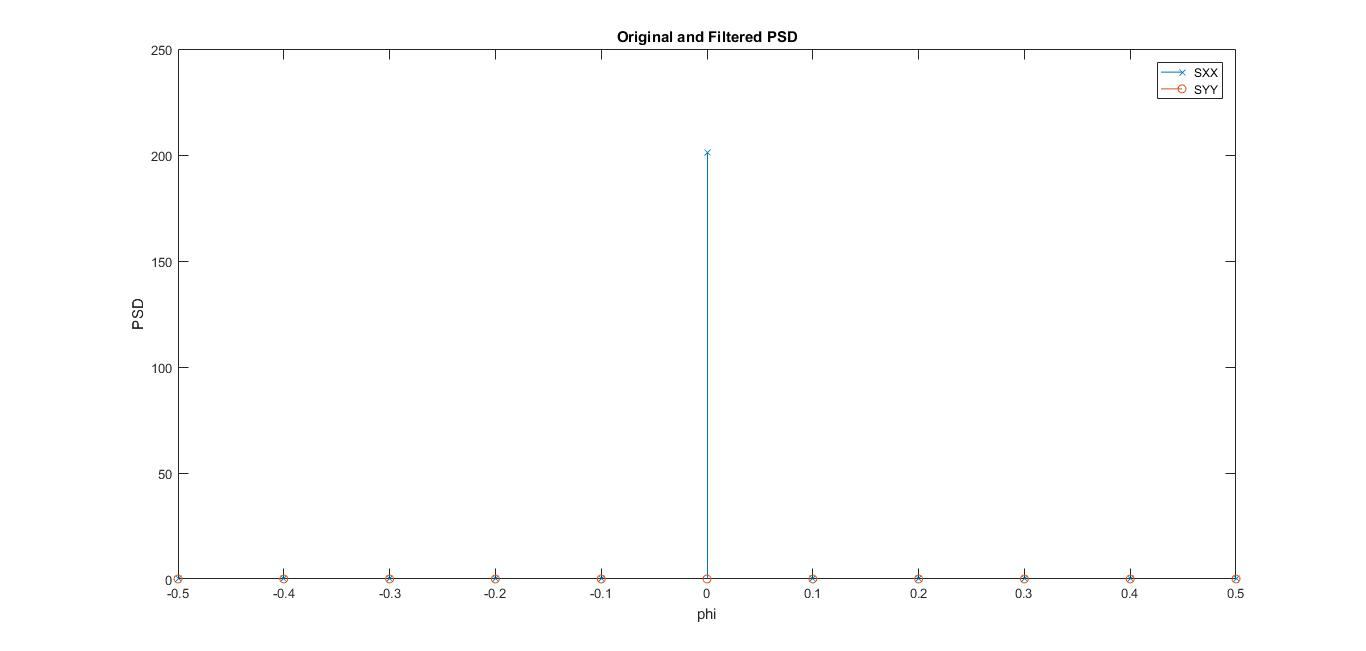
\includegraphics[scale=0.45]{q2_e}
   \caption{Original and Filtered PSD  $\mu_a = 1$,$\sigma_a^2 = 2$}\label{fig:q3}
\end{figure}
\clearpage
\newpage
\begin{figure}[h]
  \hspace*{-5cm}
   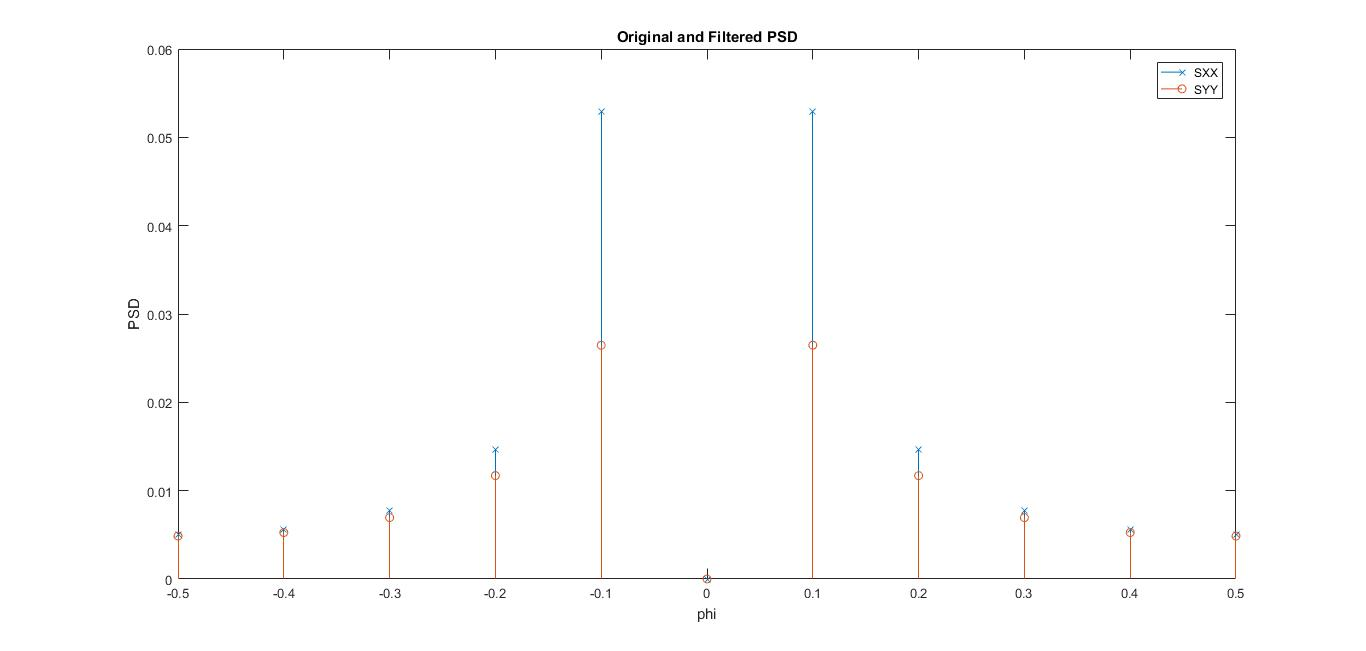
\includegraphics[scale=0.45]{q2_e_2}
   \caption{Original and Filtered PSD ignoring PSD at 0 $\mu_a = 1$,$\sigma_a^2 = 2$}\label{fig:q3}
\end{figure}
\quad \\
The  purpose of the filter is to attenuate the low frequency components of the signal. Hence, it is a \textbf{high pass} filter.
\begin{figure}[h]
  \hspace*{-5cm}
   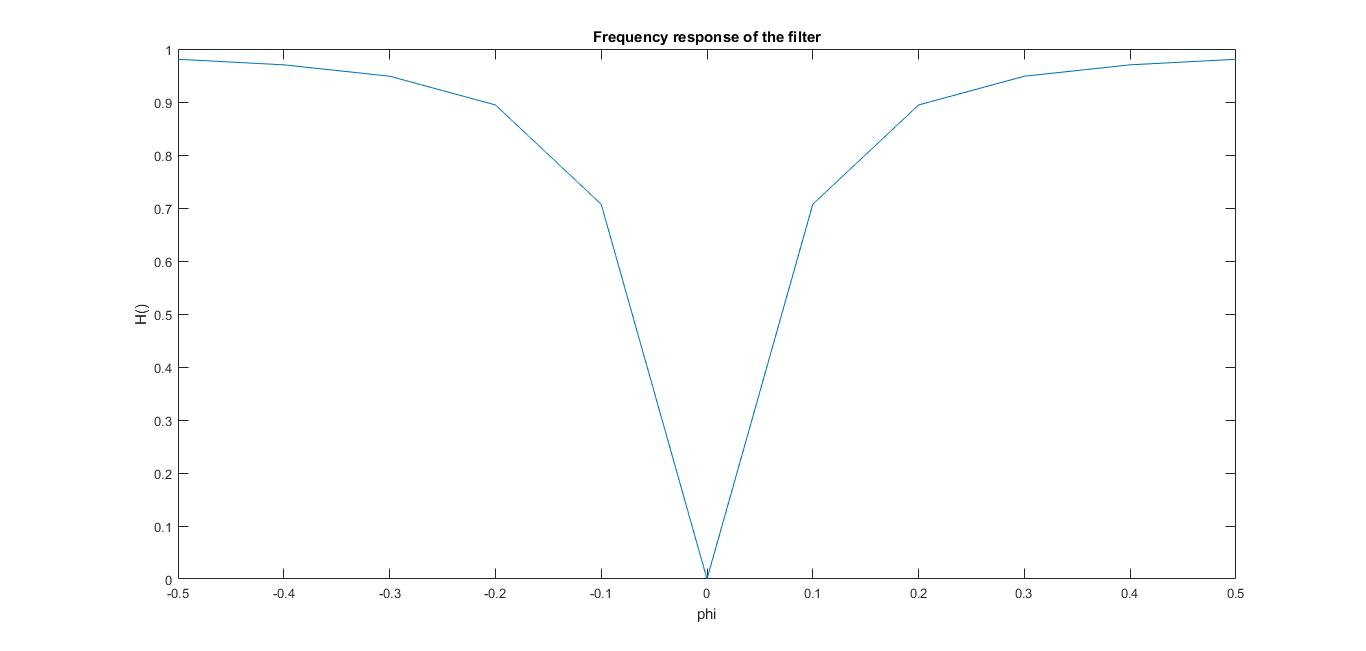
\includegraphics[scale=0.45]{q2_e_3}
   \caption{Frequency response of the filter}\label{fig:q3}
\end{figure}
\newpage
\begin{appendix}
\section*{Code Appendix}
\lstinputlisting[language=Octave]{hm12.m} 
\end{appendix}
\end{document}